\documentclass{report}[12pt]
\usepackage{amssymb}
\usepackage{amsmath}
\usepackage{geometry}
\usepackage{cite}
\usepackage[utf8]{inputenc}
\usepackage{graphicx}
\graphicspath{ {images/} }
\usepackage{float}
\usepackage{fullpage}

\usepackage{siunitx}
\usepackage{enumitem}
\usepackage{textcomp}
\usepackage{setspace}


\usepackage{color}   
\usepackage{hyperref}
\hypersetup{
    colorlinks=true, 
    linktoc=all,     
    linkcolor=blue,  
}

\author{Anurag Gupta (183230006) \\ Ponala Venkata Eswara Srisai
(183230008)\\ Sudhakar Kumar (183236001)\\ Kishan Chouhan (183230015)}
\title{Systems and Control Engineering Laboratory (SC 626) \\ Kilobotics}

\begin{document}
\maketitle
\tableofcontents
\thispagestyle{empty}
\mbox{}
\newpage

\chapter{Overview of Kilobots}
\section{Introduction}
Kilobots (Figure \ref{fig:kilobot}) are low cost, low power, tiny robots designed by Harvard University's Self Organizing Systems Research Lab with the aim of making testing collective algorithms accesible to researchers. It has following specifications:
\begin{itemize}
	\item One IR transmitter-receiver pair
	\item One ambient light sensor
	\item Two vibrators to move robot using stick and slide mechanism
	\item One onboard battery
	\item One RGB LED
\end{itemize}
\begin{figure}[H]
	\centering
	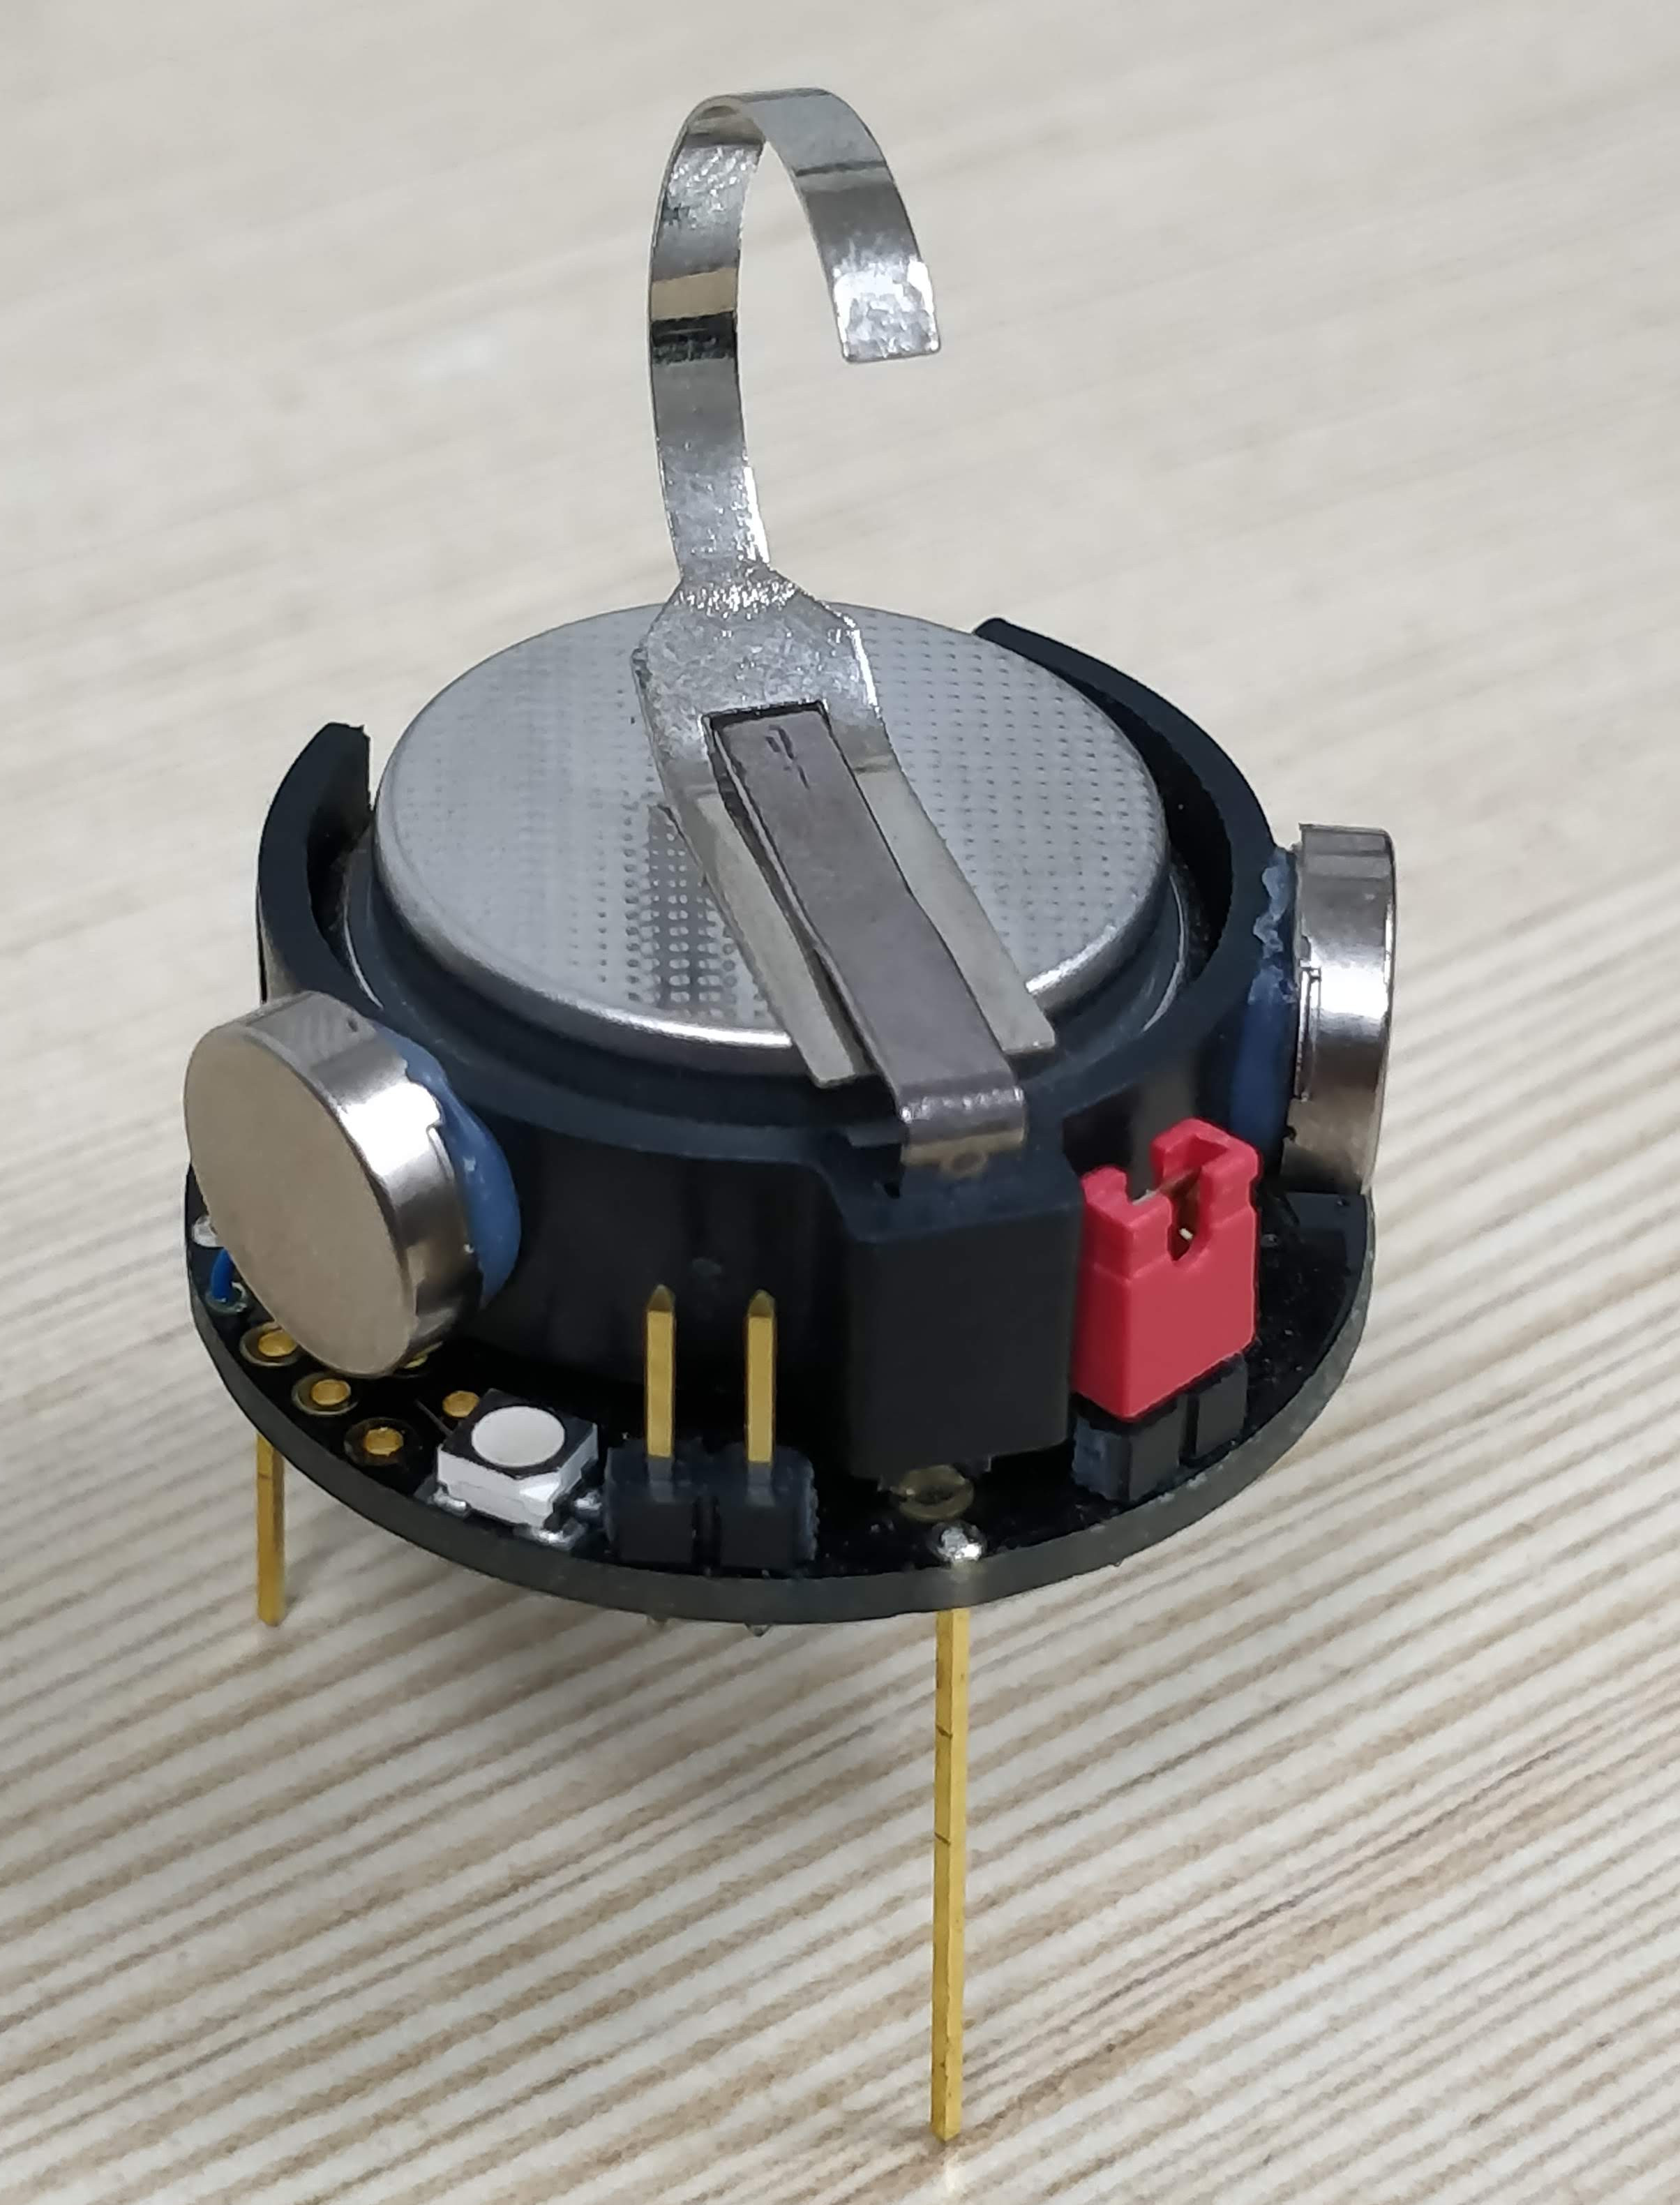
\includegraphics[scale=0.04]{images/kilobots}
	\caption{Kilobot}
	\label{fig:kilobot}
\end{figure}
A more detailed software and hardware description can be found in \cite{kilobotics_manual}.

\chapter{Kilobot Labs}

\section{Establishing communication between two Kilobots}

\section{Orbiting of Kilobots}

\section{Programming Kilobots to move towards the direction of light source}
In this part, our objective is to design an algorithm so that kilobot approaches a source of light (generated by torch light of smartphone) which may be dynamically moving with very slow speed.\\
The problem statement is similar to that of a line follower with just one onboard sensor. The algorithm for single sensor line follower goes as follows:
\begin{enumerate}
	\item Check sensor position.
	\item If sensor is on line, go to step 3 else step 4.
	\item Move right. Go to step 5.
	\item Move left.
	\item Go to step 1
\end{enumerate}
On similar lines, following a light source algorithm is implemented using flowhcart illustrated in Figure \ref{fig:move_towards_light_algorithm}.
\begin{figure}[H]
	\centering
	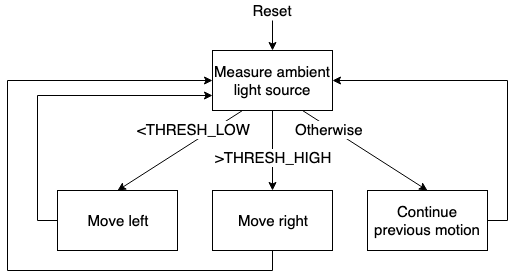
\includegraphics[scale=0.5]{images/move_towards_light_algorithm}
	\caption{Flowchart for move towards light algorithm}
	\label{fig:move_towards_light_algorithm}
\end{figure}
Abovementioned algorithm will help us understand why the robot approaches the source of light in a zig zag fashion. We cannot do significant improvement in algorithm given the limitation of onboard ambient light sensor to one.
\subsection{Demonstration}
Link to the working demo of problem statement can be accessed using link in Figure \ref{fig:move_towards_the_light}.
\begin{figure}[H]
	\centering
	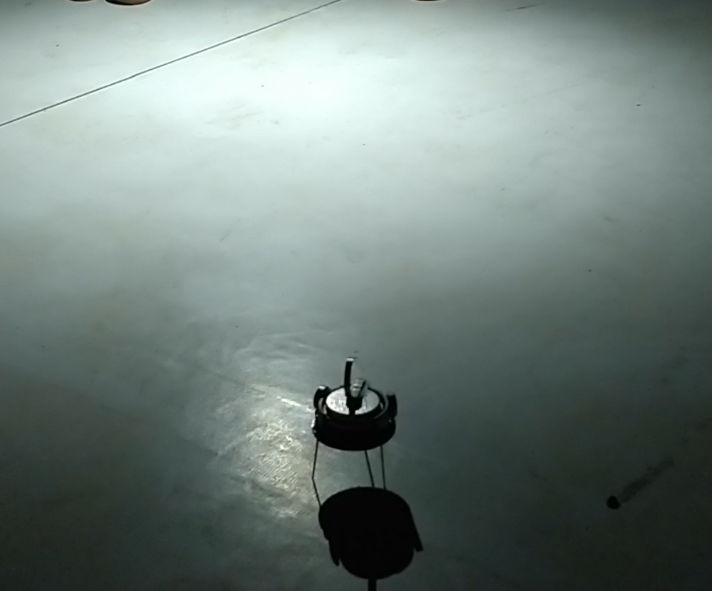
\includegraphics[scale=0.4]{images/move_towards_light}
	\caption{\href{https://www.google.com/url?sa=j&url=https\%3A\%2F\%2Fphotos.app.goo.gl\%2FnUNghDg4nJygpzUu5&uct=1551610784&usg=G0tZGJ7iMN79F5qGk1QMw5rfodM.}{Move towards the light source [Video link]}}
	\label{fig:move_towards_the_light}
\end{figure}
Different $THRESH\_LOW$ and $THRESH\_HI$ parameters were chosen to implement hysteresis behaviour, thereby, precludingjittery motion.


\section{Synchronizing phase of blinking LEDs}
\textbf{Objective}: Create a logical synchronous clock between different 
robots to allow two or more Kilobots to blink an LED in unison roughly every 4 seconds \\

\noindent A large group of decentralized closely cooperating entities, commonly called a collective or \textbf{swarm}, can work together to complete a task that is beyond the capabilities of any of its individuals \cite{rubenstein2014kilobot}. Following are the three basic swarm behaviors that Kilobots have mastered: 
\begin{enumerate}
	\item  Foraging
	\item  Formation control, and 
	\item Synchronization
\end{enumerate}
Hence, synchronization is one of the swarm behaviours which can be performed by Kilobots. It is often used when coordinating simultaneous
actions between many entities, such as robots or sensor networks.\\

\noindent For our objective, we will use a method that relies on averaging. Each Kilobot acts as an oscillator, flashing its LED in a fixed period \texttt{P}. At the same time, it continually transmits a message with its current position in the clock period (i.e. a value between \texttt{0} and \texttt{P}. In the absence of any neighbors, the Kilobot will simply blink in a fixed period, like a firefly. If the Kilobot hears neighboring Kilobots, then it receives information about their current positions in their own periods. In order to synchronize, it collects that information and uses the average to make an adjustment to its own next flashing time. \\

\noindent \textbf{Step 1}: Create a robot oscillator that flashes every 2 seconds.
\begin{verbatim}
#define PERIOD 64
uint32_t reset_time = 0;

// In Program Loop

if (kilo_ticks >= (last_reset + PERIOD)) {
   set LED to red
   last_reset = kilo_ticks
} else {
   turn LED off
}
\end{verbatim}

\noindent \textbf{Step  2}: Let the Kilobot continually transmit the current position of its clock within its ticking period (i.e. \texttt{kilo\_ticks - last\_reset}). Since we reset our clock every 64 ticks, this value will be less than 64. We want this value to be as accurate as possible, so we can read the clock in the \texttt{message\_tx} function. 
\begin{verbatim}
message_t message;

message_t *message_tx() {
    message.data[0] = kilo_ticks - last_reset; // current position in PERIOD
    message.crc = message_crc(&message);
    return &message;
}
\end{verbatim}

\noindent \textbf{Step 3}: Let the Kilobot collect the messages it hears from other neighbors. 
By comparing the its own current clock position to that of its neighbors (i.e. the first byte of the received message), a Kilobot can tell how much it is out of sync with its neighbors. Each time a new message arrives, the Kilobot will store the value of the adjustment to be made. Then, when the Kilobot completes its own time period and flashes, it will also make one big adjustment for next time's flash.

\begin{verbatim}
void message_rx(message_t *m, distance_measurement_t *d)
{
    int my_timer = kilo_ticks - last_reset;
    int rx_timer = m->data[0];
    int timer_discrepancy = my_timer - rx_timer;
    
    // reset time adjustment.
    reset_time_adjustment = reset_time_adjustment + 	rx_reset_time_adjustment;
}
\end{verbatim}

\subsection{Demonstration}

\bibliography{anurag}{}
\bibliographystyle{ieeetr}
\end{document}